%%%%%%%%%%%%%%%%%%%%%%%%%%%%%%%%%%%%%%%%%%%%%%%%%%%%%%%%%%%%%%%%%%%%%%%%%%%%%%%%%%%%%%%%%%%%%%%%%
%%%%%  Beamer Sildes  %%%%%%%%%%%%%%%%%%%%%%%%%%%%%%%%%%%%%%%%%%%%%%%%%%%%%%%%%%%%%%%%%%%%%%%%%%%
%%%%%%%%%%%%%%%%%%%%%%%%%%%%%%%%%%%%%%%%%%%%%%%%%%%%%%%%%%%%%%%%%%%%%%%%%%%%%%%%%%%%%%%%%%%%%%%%%

% https://en.wikibooks.org/wiki/LaTeX/Presentations

% \documentclass{beamer}
\documentclass{beamer}
\mode<presentation> {
% \mode<handout> {

    %%%%%  Themes  %%%%%%%%%%%%%%
    %%%%%%%%%%%%%%%%%%%%%%%%%%%%%
    % \usetheme{AnnArbor}
    % \usetheme{Antibes}
    % \usetheme{Bergen}
    % \usetheme{Berkeley}
    % \usetheme{Berlin}
    % \usetheme{CambridgeUS}
    % \usetheme{Copenhagen}
    % \usetheme{Darmstadt}
    % \usetheme{Dresden}
    % \usetheme{Frankfurt}
    % \usetheme{Goettingen}
    % \usetheme{Hannover}
    % \usetheme{Ilmenau}
    % \usetheme{JuanLesPins}
    % \usetheme{Luebeck}
    % \usetheme{Madrid}
    % \usetheme{Malmoe}
    % \usetheme{Marburg}
    % \usetheme{Montpellier}
    % \usetheme{PaloAlto}
    % \usetheme{Pittsburgh}
    % \usetheme{Rochester}
    % \usetheme{Singapore}
    % \usetheme{Szeged}
    % \usetheme{Warsaw}
    % \usetheme{boxes}
    \usetheme{default}

    %%%%%  Color Themes  %%%%%%%%
    %%%%%%%%%%%%%%%%%%%%%%%%%%%%%
    % \usecolortheme{default}
    % \usecolortheme{albatross}
    % \usecolortheme{beaver}
    % \usecolortheme{beetle}
    % \usecolortheme{crane}
    % \usecolortheme{dolphin}
    % \usecolortheme{dove}
    % \usecolortheme{fly}
    % \usecolortheme{lily}
    % \usecolortheme{orchid}
    % \usecolortheme{rose}
    % \usecolortheme{seagull}
    % \usecolortheme{seahorse}
    % \usecolortheme{whale}
    % \usecolortheme{wolverine}

    %%%%%  Outer Themes  %%%%%%%%
    %%%%%%%%%%%%%%%%%%%%%%%%%%%%%
    % \useoutertheme{infolines}
    % \useoutertheme{miniframes}
    % \useoutertheme{shadow}
    % \useoutertheme{sidebar}
    % \useoutertheme{smoothbars}
    % \useoutertheme{smoothtree}
    % \useoutertheme{split}
    % \useoutertheme{tree}

    %%%%%  Inner Themes  %%%%%%%%
    %%%%%%%%%%%%%%%%%%%%%%%%%%%%%
    % \useinnertheme{rectangles}
    % \useinnertheme{circles}
    % \useinnertheme{inmargin}
    % \useinnertheme{rounded}
}

\usepackage{amsthm}
\usepackage{amsmath}
\usepackage{amssymb}
\usepackage{array}
\usepackage[fleqn]{mathtools}
\usepackage{caption}
\usepackage{wallpaper}
\usepackage{xcolor}
\definecolor{umblue}{HTML}{00274C}
\definecolor{ummaize}{HTML}{FFCB05}
\usepackage{colortbl}
\usepackage{graphicx} 
\usepackage{pgf}
\usepackage{tikz}
\usetikzlibrary{arrows,automata}
\usepackage{url}			       
\usepackage{hyperref}

% \setbeamercolor{alerted text}{fg=orange}
% \setbeamercolor{background canvas}{bg=white}
% \setbeamercolor{block body alerted}{bg=normal text.bg!90!black}
% \setbeamercolor{block body}{bg=normal text.bg!90!black}
% \setbeamercolor{block body example}{bg=normal text.bg!90!black}
% \setbeamercolor{block title alerted}{use={normal text,alerted text},fg=alerted text.fg!75!normal text.fg,bg=normal text.bg!75!black}
% \setbeamercolor{block title}{bg=blue}
% \setbeamercolor{block title example}{use={normal text,example text},fg=example text.fg!75!normal text.fg,bg=normal text.bg!75!black}
% \setbeamercolor{fine separation line}{}
% \setbeamercolor{frametitle}{fg=brown}
% \setbeamercolor{item projected}{fg=black}
% \setbeamercolor{normal text}{bg=black,fg=yellow}
% \setbeamercolor{palette sidebar primary}{use=normal text,fg=normal text.fg}
% \setbeamercolor{palette sidebar quaternary}{use=structure,fg=structure.fg}
% \setbeamercolor{palette sidebar secondary}{use=structure,fg=structure.fg}
% \setbeamercolor{palette sidebar tertiary}{use=normal text,fg=normal text.fg}
% \setbeamercolor{section in sidebar}{fg=brown}
% \setbeamercolor{section in sidebar shaded}{fg=grey}
% \setbeamercolor{separation line}{}
% \setbeamercolor{sidebar}{bg=red}
% \setbeamercolor{sidebar}{parent=palette primary}
\setbeamercolor{structure}{bg=ummaize, fg=umblue}
% \setbeamercolor{subsection in sidebar}{fg=brown}
% \setbeamercolor{subsection in sidebar shaded}{fg=grey}
% \setbeamercolor{title}{fg=brown}
% \setbeamercolor{titlelike}{fg=brown}

% \setbeamertemplate{page number in foot}[appendixframenumber]
\setbeamertemplate{footline}[frame number]
% \setbeamertemplate{blocks}[rounded][shadow=true]
% \setbeamertemplate{background canvas}[vertical shading][bottom=white,top=structure.fg!25]
% \setbeamertemplate{sidebar canvas left}[horizontal shading][left=white!40!black,right=black]

\setbeamerfont*{footline}{family=\sffamily, size=\large}
% \setbeamerfont{title}{family=\rmfamily\addfontfeatures{Scale=1.18, Numbers={Lining, Proportional}}}
\usefonttheme[onlymath]{serif}

\beamertemplatenavigationsymbolsempty

\hypersetup{pdfstartview={Fit}} % fits the presentation to the window when first displayed

\newcommand{\XB}{\color{black}}
\newcommand{\XBB}{\color{blue}}
\newcommand{\XV}{\color{violet}}
\newcommand{\XR}{\color{red}}
\newcommand{\XUMB}{\color{umblue}}
\newcommand{\XUMM}{\color{ummaize}}

\newcommand{\ds}{\displaystyle}

% Use pause in math enviornments
\makeatletter
\renewrobustcmd{\beamer@@pause}[1][]{
  \unless\ifmeasuring@
  \ifblank{#1}
    {\stepcounter{beamerpauses}}
    {\setcounter{beamerpauses}{#1}}
  \onslide<\value{beamerpauses}->\relax
  \fi
}
\makeatother

%%%%%%%%%%%%%%%%%%%%%%%%%%%%%%%%%%%%%%%%%%%%%%%%%%%%%%%%%%%%%%%%%%%%%%%%%%%%%%%%%%%%%%%%%%%%%%%%%
%%%%%  Title Page  %%%%%%%%%%%%%%%%%%%%%%%%%%%%%%%%%%%%%%%%%%%%%%%%%%%%%%%%%%%%%%%%%%%%%%%%%%%%%%
%%%%%%%%%%%%%%%%%%%%%%%%%%%%%%%%%%%%%%%%%%%%%%%%%%%%%%%%%%%%%%%%%%%%%%%%%%%%%%%%%%%%%%%%%%%%%%%%%

\title[Introduction to Community Detection in Networks]{Introduction to Community Detection in Networks via Modularity Maximization}
\author{\XV\textit{\large{\href{https://github.com/casonk}{Cason Konzer}}}\XB}
\institute[UM FLINT]{\normalsize{\textit{casonk@umich.edu}}}
\titlegraphic{\includegraphics[scale = 0.5]{C:/OneDriveSchool/OneDrive - Umich/Math/Classes/Fall_2022/Capstone/Deliverables/final_slides/University_of_Michigan_Flint.png}}
\date[]{\today} 

\begin{document}

\begin{frame}
    \titlepage
\end{frame}


%%%%%%%%%%%%%%%%%%%%%%%%%%%%%%%%%%%%%%%%%%%%%%%%%%%%%%%%%%%%%%%%%%%%%%%%%%%%%%%%%%%%%%%%%%%%%%%%%
%%%%%  Begin Slides  %%%%%%%%%%%%%%%%%%%%%%%%%%%%%%%%%%%%%%%%%%%%%%%%%%%%%%%%%%%%%%%%%%%%%%%%%%%%
%%%%%%%%%%%%%%%%%%%%%%%%%%%%%%%%%%%%%%%%%%%%%%%%%%%%%%%%%%%%%%%%%%%%%%%%%%%%%%%%%%%%%%%%%%%%%%%%%

%%%%%  Introduction  %%%%%%%%%%%%%%%%%%%%%%%%%%%%%%%%%%%%%%%%%%%%%%%%%%%%%%%%%%%%%%%%%%%%%%%%%%%%

\section{Introduction}

\begin{frame}

    \frametitle{Introduction}

    What exactly is a network?\pause

    \vspace{2.5mm}
    \begin{itemize}
        \item A network is a group of objects in which we call nodes.\pause
        \item[$\diamond$] for example web pages, authors, and transit hubs.\pause
        \item[$\diamond$] the objects may have attributes such as age, expertise, and city.\pause
        \item Objects are then connected by edges which represent node relations.\pause
        \item[$\diamond$] for example references, and transit paths.\pause
        \item[$\diamond$] the connections may also have attributes such as hyperlink, road, and shipping lane.   
    \end{itemize}

\end{frame}

%%%%%  Examples  %%%%%%%%%%%%%%%%%%%%%%%%%%%%%%%%%%%%%%%%%%%%%%%%%%%%%%%%%%%%%%%%%%%%%%%%%%%%%%%%

\begin{frame}

    \frametitle{Example: Web Pages}
    \includegraphics[width=\textwidth]{C:/OneDriveSchool/OneDrive - Umich/Math/Classes/Fall_2022/Capstone/Deliverables/final_slides/Web_Page_Example.PNG}

\end{frame}

\begin{frame}

    \frametitle{Example: Social Media}
    \includegraphics[width=\textwidth]{C:/OneDriveSchool/OneDrive - Umich/Math/Classes/Fall_2022/Capstone/Deliverables/final_slides/Social_Media_Example.PNG}

\end{frame}

\begin{frame}

    \frametitle{Example: Transit}
    \includegraphics[width=\textwidth]{C:/OneDriveSchool/OneDrive - Umich/Math/Classes/Fall_2022/Capstone/Deliverables/final_slides/Transit_Example.PNG}

\end{frame}

%%%%%  Communities  %%%%%%%%%%%%%%%%%%%%%%%%%%%%%%%%%%%%%%%%%%%%%%%%%%%%%%%%%%%%%%%%%%%%%%%%%%%%%

\begin{frame}

    \frametitle{Communities}

    What is a community within a network?\pause

    \vspace{2.5mm}
    \begin{itemize}
        \item Communities are partitions of the network.\pause
        \item[$\diamond$] every node should fall into at least one community.\pause
        \item[$\diamond$] communities may be disjoint, hierarchical, or overlapping.\pause
        \item[$\ast$] think of sets.\pause
        \item We expect nodes within a community to share similar attributes.\pause
        \item[$\diamond$] often communities are considered to have a high density of internal edges compared to that of external edges. 
    \end{itemize}

\end{frame}

\begin{frame}

    \frametitle{Community Examples}
    \includegraphics[width=\textwidth]{C:/OneDriveSchool/OneDrive - Umich/Math/Classes/Fall_2022/Capstone/Deliverables/final_slides/Community_Example.PNG}

\end{frame}

%%%%%  Motivation  %%%%%%%%%%%%%%%%%%%%%%%%%%%%%%%%%%%%%%%%%%%%%%%%%%%%%%%%%%%%%%%%%%%%%%%%%%%%%%

\begin{frame}

    \frametitle{Motivation}

    Why study communities in networks?\pause

    \vspace{2.5mm}
    \begin{itemize}
        \item Community detection has many applications.\pause
        \item[$\diamond$] often it can be used for recommendation purposes.\pause
        \item[$\ast$] finding web pages with similar topics.\pause
        \item[$\ast$] finding friends within your social circle.\pause
        \item[$\ast$] finding groups of bad actors.\pause
        \item[$\ast$] finding products the community as a whole may like.\pause
        \item[$\diamond$] community connecting edges may be of concern.\pause
        \item[$\ast$] finding roads in need of additional lanes.\pause
        \item[$\ast$] finding authors with cross domain knowledge.\pause
        \item[$\diamond$] etc. 
    \end{itemize}

\end{frame}

%%%%%  Methods  %%%%%%%%%%%%%%%%%%%%%%%%%%%%%%%%%%%%%%%%%%%%%%%%%%%%%%%%%%%%%%%%%%%%%%%%%%%%%%%%%%

\begin{frame}

    \frametitle{Methods}

    There are many methods in which one can find communities. Some examples include the following.\pause

    \vspace{2.5mm}
    \begin{itemize}
        \item Shortest Path Betweeness.\pause
        \item Random Walk Betweeness.\pause
        \item Modularity Maximization.\pause
        \item Maximum Liklihood Estimation. 
    \end{itemize}

\end{frame}

\begin{frame}

    \frametitle{Method Evaluation}

    How might we choose a method in application? In general we must consider two criteria.\pause

    \vspace{2.5mm}
    \begin{itemize}
        \item Accuracy.\pause
        \item[$\diamond$] How close are detected communities to their ground truth?\pause
        \item Complexity.\pause
        \item[$\diamond$] How long does it take to detect communities?\pause
        \item[$\ast$] How big of a network can the method run on?\pause
    \end{itemize}

    \vspace{2.5mm}
    Today we will focus on Modularity Maximization methods. 

\end{frame}

%%%%%  Nomenclature  %%%%%%%%%%%%%%%%%%%%%%%%%%%%%%%%%%%%%%%%%%%%%%%%%%%%%%%%%%%%%%%%%%%%%%%%%%%%

\begin{frame}

    \frametitle{Nomenclature}

    Let us define basic terminology.\pause

    \vspace{5mm}
    \begin{itemize}
        \item Let $ n $ be the number of nodes in the network.\pause
        \item Let $ m $ be the number of edges in the network.\pause
        \item Let $ s = 2m $ be the number of spokes (edge ends) in the network.\pause
        \item Let $ k_{i} $ be the number of spokes incident upon a node $ i $.\pause
        \item Let $ k_{i}^{in} $ be the number of inbound edges for a node $ i $.\pause
        \item Let $ k_{i}^{out} $ be the number of outbound edges for a node $ i $.\pause
        \item Let $ A $ be an adjacency matrix with entries $ A_{i, j} $ representing the number of spokes connecting nodes $ i $ and $ j $.\pause
        \item Let $ \vec{A} $ be a directed adjacency matrix with entries $ \vec{A}_{i, j} $ representing an edge from node $ i $ to $ j $. 
    \end{itemize}

\end{frame}

\begin{frame}

    \frametitle{Network Types}

    Networks can take on the following types.\pause

    \vspace{2.5mm}
    \begin{itemize}
        \item Undirected Graph.\pause
        \item[$\diamond$] An edge from node $ i $ to $ j $ implies an edge from node $ j $ to $ i $.\pause
        \item Weighted or Multi-Graph.\pause
        \item[$\diamond$] Multiple edges can run between two nodes, or otherwise edges can be given weights as an attribute.\pause
        \item Directed Graph.\pause
        \item[$\diamond$] An edge from node $ i $ to $ j $ does not imply an edge from node $ j $ to $ i $.
    \end{itemize}

\end{frame}

%%%%%  Network Modeling  %%%%%%%%%%%%%%%%%%%%%%%%%%%%%%%%%%%%%%%%%%%%%%%%%%%%%%%%%%%%%%%%%%%%%%%%%

\section{Modeling}

\begin{frame}

    \frametitle{Network Modeling}

    In graph theory there are many ways one can model networks.\pause

    \vspace{2.5mm}
    \begin{itemize}
        \item Erdős–Rényi Model.\pause
        \item Exponential Random Graph Model.\pause
        \item Stochastic Block Model.\pause
        \item Configuration Model.\pause
    \end{itemize}
    \vspace{2.5mm}

    In general different models generate graphs based on an underlying theory of how edges are formed between nodes. 
    Modularity Maximization leverages the configuration model. 

\end{frame}

\begin{frame}

    \frametitle{Configuration Model}

    The configuration model leverages a set degree distribution.\pause

    \vspace{2.5mm}
    \begin{itemize}
        \item In real-world graphs, the degree distribution is given.\pause
        \item Graphs generated from the configuration model must obey the set degree distribution.\pause
        \item[$\diamond$] many graphs may be possible with the same degree distribution.\pause
        \item[$\diamond$] the model creates edges between nodes based on the probability of them existing.\pause
        \item[$\ast$] this probability is derived from the degree distribution.  
    \end{itemize}

\end{frame}

\begin{frame}

    \frametitle{Configuration Model Features}

    The configuration model provides us with some nice features.\pause

    \vspace{2.5mm}
    \begin{itemize}
        \item The total number of spokes will be, $ \ds \sum_{i}^{n} k_{i} = s $.\pause
        \item The total number of edges will be, $ \ds \sum_{i}^{n} k_{i}^{out} = \sum_{i}^{n} k_{i}^{in} = m $.\pause
        \item The number of ways to connect spokes (form edges) between two distinct nodes $ i,j $ in an undirected network is $ \ds k_{i} k_{j} $.\pause
        \item The number of ways to from self loops for a node $ i $ is $ \ds k_{i}(k_{i} - 1) $. \pause
        \item The number of ways to form an edge from node $ i $ to node $ j $ in a directed network is $ \ds k_{i}^{out} k_{j}^{in} $.
    \end{itemize}


\end{frame}

%%%%%  Expectation  %%%%%%%%%%%%%%%%%%%%%%%%%%%%%%%%%%%%%%%%%%%%%%%%%%%%%%%%%%%%%%%%%%%%%%%%%%%%%%

\begin{frame}

    \frametitle{Spoke/Edge Expectation}

    Building upon the features of the configuration model, let us define the expected number of spokes/edges between two nodes.\pause

    \vspace{2.5mm}
    First let us note the following relating to the number of ways to connect nodes in networks.\pause

    \vspace{2.5mm}
    \begin{itemize}
        \item $ \ds \sum_{i}^{n} k_{i} \sum_{j}^{n} k_{j} = s^{2} $.\pause
        \item[$\diamond$] undirected case (spokes).\pause
        \item $ \ds \sum_{i}^{n} k_{i}^{out} \sum_{j}^{n} k_{j}^{in} = m^{2} $.\pause
        \item[$\diamond$] directed case (edges). 
    \end{itemize}

\end{frame}

\begin{frame}

    \frametitle{Spoke/Edge Expectation}

    When summing over the expected number of spokes for each undirected node pair we should get the total number of spokes ($ s $).\pause 

    \vspace{2.5mm}
    When summing over the expected number of edges for each directed node pair we should get the total number of edges ($ m $).\pause 

    \vspace{2.5mm}
    Building upon the previous slide we can retrieve the expected number of spokes/edges $ \mathbb{E}_{i, j} $ and $ \vec{\mathbb{E}}_{i, j} $ in an undirected and directed network.\pause

    \vspace{2.5mm}
    \begin{itemize}
        \item $ \ds \mathbb{E}_{i, j \ne i} = \frac{k_{i} k_{j}}{s - 1} $.\pause
        \item $ \ds \mathbb{E}_{i, i} = \frac{k_{i} (k_{i} - 1)}{s - 1} $.\pause
        \item $ \ds \vec{\mathbb{E}}_{i, j} = \frac{k_{i}^{out} k_{j}^{in}}{m} $. 
    \end{itemize}

\end{frame}

\begin{frame}

    \frametitle{Proof of Spoke Expectation (Undirected)}

    \begin{flalign*}
        & \ds \sum_{i, j}^{n} \mathbb{E}_{i, j} = \sum_{i, j \ne i}^{n} \mathbb{E}_{i, j} + \sum_{i}^{n} \mathbb{E}_{i, i} \\ \pause
        &= \sum_{i, j \ne i}^{n} \frac{k_{i} k_{j}}{s - 1} + \sum_{i}^{n} \frac{k_{i} (k_{i} - 1)}{s - 1} \\ \pause
        &= \frac{1}{s - 1} \left[ \sum_{i}^{n} k_{i} \sum_{j \ne i}^{n} k_{j} + \sum_{i}^{n} k_{i} \sum_{i}^{n} k_{i} - \sum_{i}^{n} k_{i} \right] \\ \pause
        &= \frac{1}{s - 1} \left[ \sum_{i}^{n} k_{i} \sum_{j}^{n} k_{j} - s \right] \\ \pause
        &= \frac{s^{2} - s}{s - 1} \pause = \frac{s(s - 1)}{s - 1} \pause = s
    \end{flalign*}

\end{frame}

\begin{frame}

    \frametitle{Proof of Edge Expectation (Directed)}

    \begin{flalign*}
        & \ds \sum_{i, j}^{n} \vec{\mathbb{E}}_{i, j} = \sum_{i, j}^{n} \frac{k_{i}^{out} k_{j}^{in}}{m} \\ \pause
        &= \frac{1}{m} \left[ \sum_{i}^{n} k_{i}^{out} \sum_{j}^{n} k_{j}^{in} \right] \\ \pause
        &= \frac{m^{2}}{m} \pause = m
    \end{flalign*}

\end{frame}

%%%%%  Modularity  %%%%%%%%%%%%%%%%%%%%%%%%%%%%%%%%%%%%%%%%%%%%%%%%%%%%%%%%%%%%%%%%%%%%%%%%%%%%%%%

\section{Modularity}

\begin{frame}

    \frametitle{Modularity (Undirected)}

    Modularity is meant to measure the goodness of community partitions, under the assumption that communities have a high density of internal edges.\pause

    \vspace{2.5mm}
    \begin{itemize}
        \item $ Q = \% \ internal \ edges - Expected \ \% \ internal \ edges $.\pause
        \item $ \ds \delta(c_{i}, c_{j}) =
            \begin{cases}
                1 & i \ \& \ j \ are \ in \ the \ same \ community \\ \pause
                0 & else
            \end{cases}
            $.\pause
        \item Note: $ \delta(c_{i}, c_{i}) = 1 $.\pause
    \end{itemize}

    \vspace{2.5mm}
    \begin{multline*}
        \ds Q = \frac{1}{s} \Biggl[ \sum_{i, j \ne i}^{n} \left( A_{i, j} - \frac{k_{i}k_{j}}{s - 1} \right) \delta(c_{i}, c_{j}) \\ 
        +  \sum_{i}^{n} \left( A_{i,i} - \frac{k_{i}(k_{i} - 1)}{s - 1} \right) \Biggr].
    \end{multline*}

\end{frame}

\begin{frame}

    \frametitle{Modularity Simplified (Undirected)}

    Heuristics:\pause
    \begin{enumerate}
        \item As networks grow large the subtraction of $ 1 $ from the number of possible spoke to spoke connections becomes negligible.\pause
        \item The number of self edges is proportionally small compared to the total number of edges, and can be treated as if the repeated nodes are distinct. \pause
    \end{enumerate}

    Simplifications:\pause
    \begin{enumerate}
        \item $ \ds \frac{k_{i}k_{j}}{s - 1} \approx \frac{k_{i}k_{j}}{s} $.\pause
        \item $ k_{i}(k_{i} - 1) \approx k_{i}^{2} $.\pause
    \end{enumerate}

    \begin{flalign*}
        & \ds Q = \frac{1}{s} \Biggl[ \sum_{i, j}^{n} \left( A_{i, j} - \frac{k_{i}k_{j}}{s} \right) \delta(c_{i}, c_{j})  \Biggr]. 
    \end{flalign*}

\end{frame}

\begin{frame}

    \frametitle{Modularity (Directed)}

    Only a slight modification is needed to extend modularity to directed networks.\pause

    \vspace{2.5mm}
    This modification follows from previous work and is to use $ \vec{\mathbb{E}}_{i, j} $ for edge expectation rather than $ \mathbb{E}_{i, j} $\pause

    \vspace{2.5mm}
    \begin{flalign*}
        & \ds \vec{Q} = \frac{1}{m} \Biggl[ \sum_{i, j}^{n} \left( \vec{A}_{i, j} - \frac{k_{i}^{out}k_{j}^{in}}{m} \right) \delta(c_{i}, c_{j})  \Biggr].
    \end{flalign*}\pause

    \vspace{2.5mm}
    If one likes modularity can be written in the following form:\pause

    \vspace{2.5mm}
    \begin{flalign*}
        & \ds \vec{Q} = \frac{1}{m} \Biggl[ \sum_{i, j}^{n} \left( \vec{A}_{i, j} - \vec{\mathbb{E}}_{i, j} \right) \delta(c_{i}, c_{j})  \Biggr].
    \end{flalign*}

\end{frame}

%%%%%  Algorithms  %%%%%%%%%%%%%%%%%%%%%%%%%%%%%%%%%%%%%%%%%%%%%%%%%%%%%%%%%%%%%%%%%%%%%%%%%%%%%%%

\section{Algorithms}

\begin{frame}

    \frametitle{Introduction to Modularity Maximization}

    Initially, let us assume all nodes belong to a distinct community.\pause

    \vspace{2.5mm}
    From here we can consider changes in modularity based on reassigning node communities.\pause

    \vspace{2.5mm}
    In an iterative fashion, we can performed the reassignment with the greatest increase in modularity.\pause

    \vspace{2.5mm}
    One note on modularity maximization methods is that they detect disjoint communities, so it has a decreased accuracy for networks with underlying hierarchical or overlapping mechanics. 

\end{frame}

\begin{frame}

    \frametitle{Complexity Optimization in Modularity Maximization [1/2]}

    In general, modularity maximization techniques are often used due to their ability to analyze massive networks (millions of nodes).\pause

    \vspace{2.5mm}
    In order to have a reasonable runtime, there are a few steps in which we can optimize.\pause

    \vspace{2.5mm}
    \begin{itemize}
        \item How we reassign communities.\pause
        \item How we calculate modularity changes.\pause
        \item When we stop iterating. 
    \end{itemize}

\end{frame}

\begin{frame}

    \frametitle{Complexity Optimization in Modularity Maximization [2/2]}

    How might we go about such optimizations?

    \vspace{2.5mm}
    \begin{itemize}
        \item Reassign multiple node communities in each iteration.\pause
        \item Consider reassignments only within node neighborhoods (the neighbors of a node are all nodes in which it shares an edge).\pause
        \item Cache relevant values (node degrees, expectations) rather than computing during runtime.\pause
        \item Halt the algorithm once the highest possible change in modularity is below a set threshold. 
    \end{itemize}

\end{frame}

%%%%%  Examples

\tikzset{every loop/.style={min distance=5mm}}
\begin{frame}

    \frametitle{Example: Network}
    \begin{figure}[t]
        \centering
        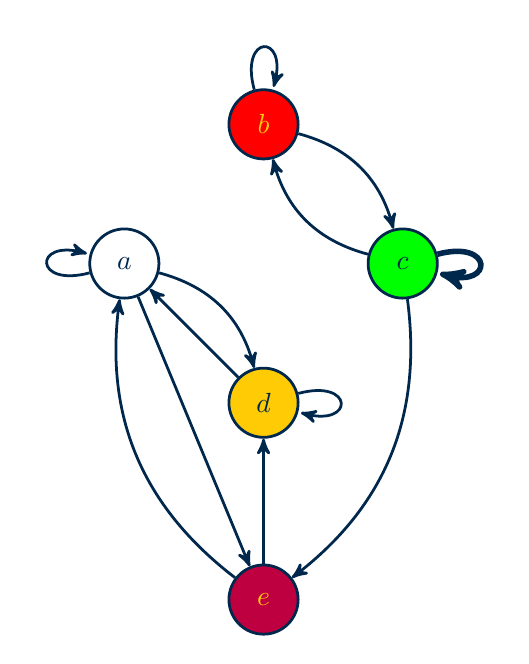
\begin{tikzpicture}[->,>=stealth',auto,node distance=2.5cm,semithick,line width=1pt]
            \tikzstyle{be}=[color=umblue]
            \tikzstyle{be2}=[color=umblue,line width=2pt]
            
            \node[state,fill=white,draw=umblue,text=umblue]   (A)                    {$a$};
            \node[state,fill=red,draw=umblue,text=ummaize]    (B) [above right of=A] {$b$};
            \node[state,fill=ummaize,draw=umblue,text=umblue] (D) [below right of=A] {$d$};
            \node[state,fill=green,draw=umblue,text=umblue]   (C) [below right of=B] {$c$};
            \node[state,fill=purple,draw=umblue,text=ummaize] (E) [below of=D]       {$e$};
            
            \path   (A) edge [be,loop  left]   node {} (A)
                        edge [be]              node {} (E)
                        edge [be, bend left]   node {} (D)
                    (B) edge [be, loop above]  node {} (B)
                        edge [be, bend  left]  node {} (C)
                    (C) edge [be2, loop right] node {} (C)
                        edge [be, bend  left]  node {} (E)
                        edge [be, bend  left]  node {} (B)
                    (D) edge [be, loop right]  node {} (D)
                        edge [be]              node {} (A)
                    (E) edge [be, bend  left]  node {} (A)
                        edge [be]              node {} (D);
            
        \end{tikzpicture}
    \end{figure}  

\end{frame}

\begin{frame}

    \frametitle{Example: Adjacency Matrix}

    \begin{center}
        \begin{tabular}{l | c c c c c} 
            $ \vec{A} $ & $ a $ & $ b $ & $ c $ & $ d $ & $ e $ \\
            \hline
            $ a $ & $ 1 $ & $ 0 $ & $ 0 $ & $ 1 $ & $ 1 $ \\
            $ b $ & $ 0 $ & $ 1 $ & $ 1 $ & $ 0 $ & $ 0 $ \\
            $ c $ & $ 0 $ & $ 1 $ & $ 2 $ & $ 0 $ & $ 1 $ \\
            $ d $ & $ 1 $ & $ 0 $ & $ 0 $ & $ 1 $ & $ 0 $ \\
            $ e $ & $ 1 $ & $ 0 $ & $ 0 $ & $ 1 $ & $ 0 $ \\
        \end{tabular}
    \end{center}\pause

    \vspace{2.5mm}
    The adjacency matrix is the expected form computers will store networks in. 

\end{frame}

\begin{frame}

    \frametitle{Example: Out-Degree Calculations}

    \begin{center}
        \begin{tabular}{l | c c c c c} 
            $ \vec{A} $ & $ a $ & $ b $ & $ c $ & $ d $ & $ e $ \\
            \hline
            \rowcolor{ummaize}
            $ a $ & $ 1 $ & $ 0 $ & $ 0 $ & $ 1 $ & $ 1 $ \\
            $ b $ & $ 0 $ & $ 1 $ & $ 1 $ & $ 0 $ & $ 0 $ \\
            $ c $ & $ 0 $ & $ 1 $ & $ 2 $ & $ 0 $ & $ 1 $ \\
            $ d $ & $ 1 $ & $ 0 $ & $ 0 $ & $ 1 $ & $ 0 $ \\
            $ e $ & $ 1 $ & $ 0 $ & $ 0 $ & $ 1 $ & $ 0 $ \\
        \end{tabular}
    \end{center}\pause

    \vspace{2.5mm}
    $ \ds k_{a}^{out} = 1 + 0 + 0 + 1 + 1 = 3 $. 

\end{frame}

\begin{frame}

    \frametitle{Example: In-Degree Calculations}

    \begin{center}
        \begin{tabular}{l | >{\columncolor{ummaize}}c c c c c} 
            $ \vec{A} $ & $ a $ & $ b $ & $ c $ & $ d $ & $ e $ \\
            \hline
            $ a $ & $ 1 $ & $ 0 $ & $ 0 $ & $ 1 $ & $ 1 $ \\
            $ b $ & $ 0 $ & $ 1 $ & $ 1 $ & $ 0 $ & $ 0 $ \\
            $ c $ & $ 0 $ & $ 1 $ & $ 2 $ & $ 0 $ & $ 1 $ \\
            $ d $ & $ 1 $ & $ 0 $ & $ 0 $ & $ 1 $ & $ 0 $ \\
            $ e $ & $ 1 $ & $ 0 $ & $ 0 $ & $ 1 $ & $ 0 $ \\
        \end{tabular}
    \end{center}\pause

    \vspace{2.5mm}
    $ k_{a}^{in} = 1 + 0 + 0 + 1 + 1 = 3 $. 

\end{frame}

\begin{frame}

    \frametitle{Example: All Degree Calculations}

    \begin{center}
        \begin{tabular}{l | c c c c c} 
            $ i           $ & $ a $ & $ b $ & $ c $ & $ d $ & $ e $ \\
            \hline
            \rowcolor{ummaize}
            $ k_{i}^{out} $ & $ 3 $ & $ 2 $ & $ 4 $ & $ 2 $ & $ 2 $ \\
            \rowcolor{ummaize}
            $ k_{i}^{in}  $ & $ 3 $ & $ 2 $ & $ 3 $ & $ 3 $ & $ 2 $ \\
            $ k_{i}       $ & $ 6 $ & $ 4 $ & $ 7 $ & $ 5 $ & $ 4 $ \\
        \end{tabular}
    \end{center}\pause

    \vspace{2.5mm}
    $ m = 3 + 2 + 4 + 2 + 2 \pause = 3 + 2 + 3 + 3 + 2 \pause = 13 $. 

\end{frame}

\begin{frame}

    \frametitle{Example: Modularity Calculation [1/2]}

    We need only consider the diagonal of the adjacency matrix as all node pairs but the self pair are not in the same community.\pause

    \vspace{2.5mm}
    \begin{multline*}
        \ds \vec{Q} = \frac{1}{m} \Bigl[ (\vec{A}_{a, a} - \vec{\mathbb{E}}_{a, a}) + (\vec{A}_{b, b} - \vec{\mathbb{E}}_{b, b}) \\
        + (\vec{A}_{c, c} - \vec{\mathbb{E}}_{c, c}) + (\vec{A}_{d, d} - \vec{\mathbb{E}}_{d, d}) + (\vec{A}_{e, e} - \vec{\mathbb{E}}_{e, e}) \Bigr].
    \end{multline*}\pause

    \vspace{2.5mm}
    \begin{multline*}
        \ds \vec{Q} = \frac{1}{13} \Bigl[ (1 - \frac{3 \cdot 3}{13}) + (1 - \frac{2 \cdot 2}{13}) \\
        + (2 - \frac{4 \cdot 3}{13}) + (1 - \frac{2 \cdot 3}{13}) + (0 - \frac{2 \cdot 2}{13}) \Bigr].
    \end{multline*}

\end{frame}

\begin{frame}

    \frametitle{Example: Modularity Calculation [2/2]}

    \begin{flalign*}
        & \ds \vec{Q} = \frac{1}{13} \Bigl[ \frac{4}{13} + \frac{9}{13} + \frac{14}{13} + \frac{7}{13} - \frac{4}{13} \Bigr]. \\ \pause
        & \vec{Q} = \frac{1}{13} \cdot \frac{30}{13} \pause = \frac{30}{169}.
    \end{flalign*}

\end{frame}

\begin{frame}

    \frametitle{Modularity Maximization Algorithm [1/2]}

    How does a modularity maximization algorithm operate in practice?\pause

    \vspace{2.5mm}
    Typically, community reassignments are realized as node merges.\pause

    \vspace{2.5mm}
    By doing so we can treat merged nodes as meta nodes, and form a new adjacency matrix with them.\pause

    \vspace{2.5mm} 
    As a result we need only update the cached values which change. 

\end{frame}

\begin{frame}

    \frametitle{Modularity Maximization Algorithm [2/2]}

    To calculate $ \Delta \vec{Q} $ we need only consider changes in modularity resulting from the node merge.\pause

    \vspace{2.5mm}
    For our adjacency matrix this is just a row and column merge.\pause

    \vspace{2.5mm}
    Similarly, for recalculating $ k_{i}^{out} $ and $ k_{i}^{in} $ we need only one addition.\pause

    \vspace{2.5mm} 
    Last, we will only consider merges for nodes which are neighbors. 

\end{frame}

\begin{frame}

    \frametitle{Example: Neighborhoods}

    Form our example graph we can create a neighborhood table as follows.\pause

    \vspace{2.5mm}
    \begin{center}
        \begin{tabular}{l | c} 
            $ i           $ & $ neighborhood $ \\
            \hline
            $ a $ & $ \{d, e\}    $ \\
            $ b $ & $ \{c\}       $ \\
            $ c $ & $ \{b, e\}    $ \\
            $ d $ & $ \{a, e\}    $ \\
            $ e $ & $ \{a, c, e\} $ \\
        \end{tabular}
    \end{center}\pause

    \vspace{2.5mm}
    Further, we can derive all node merges which must be considered.\pause

    \vspace{2.5mm}
    \begin{center}
        $ \{a, d\}, \{a, e\}, \{b, c\}, \{c, e\}, \{d, e\} $.
    \end{center}\pause

    \vspace{2.5mm}
    The merges we need consider should be much less that the $ \ds \binom{n}{2} $ node pairs.  

\end{frame}

\begin{frame}

    \frametitle{Example: $ \Delta \vec{Q} $ Calculation [1/2]}

    We will choose the node merge with the best change $ \Delta \vec{Q} $.\pause

    \vspace{2.5mm}
    \begin{center}
        \begin{tabular}{l | c c c c c} 
            $ merge    $ & $ A_{i,i} $ & $ A_{j,j} $ & $ A_{i,j} $ & $ A_{j,i} $ & $ A_{i',i'} $  \\
            \hline
            $ \{a, d\} $ & $ 1 $ & $ 1 $ & $ 1 $ & $ 1 $ & $ 4 $ \\
            $ \{a, e\} $ & $ 1 $ & $ 0 $ & $ 1 $ & $ 1 $ & $ 3 $ \\
            $ \{b, c\} $ & $ 1 $ & $ 2 $ & $ 1 $ & $ 1 $ & $ 5 $ \\
            $ \{c, e\} $ & $ 2 $ & $ 0 $ & $ 1 $ & $ 0 $ & $ 3 $ \\
            $ \{d, e\} $ & $ 1 $ & $ 0 $ & $ 0 $ & $ 1 $ & $ 2 $ \\
        \end{tabular}
    \end{center}\pause

    \begin{center}
        \begin{tabular}{l | c c c c c c} 
            $ merge    $ & $ k_{i}^{out} $ & $ k_{j}^{out} $ & $ k_{i'}^{out} $ & $ k_{i}^{in} $ & $ k_{j}^{in} $ & $ k_{i'}^{in} $ \\
            \hline
            $ \{a, d\} $ & $ 3 $ & $ 2 $ & $ 5 $ & $ 3 $ & $ 3 $ & $ 6 $ \\
            $ \{a, e\} $ & $ 3 $ & $ 2 $ & $ 5 $ & $ 3 $ & $ 2 $ & $ 5 $ \\
            $ \{b, c\} $ & $ 2 $ & $ 4 $ & $ 6 $ & $ 2 $ & $ 3 $ & $ 5 $ \\
            $ \{c, e\} $ & $ 4 $ & $ 2 $ & $ 6 $ & $ 3 $ & $ 2 $ & $ 5 $ \\
            $ \{d, e\} $ & $ 2 $ & $ 2 $ & $ 4 $ & $ 3 $ & $ 2 $ & $ 5 $ \\
        \end{tabular}
    \end{center}\pause

    \vspace{2.5mm}
    Where $ i' $ is the new meta node formed from merging nodes $ i $ and $ j $.

\end{frame}

\begin{frame}

    \frametitle{Example: $ \Delta \vec{Q} $ Calculation [2/2]}

    Let $ \partial \vec{Q}_{i}, \partial \vec{Q}_{j}, \partial \vec{Q}_{i'} $ denote the contribution to modularity by the communities $ i, j, $ and $ i' $ respectively.\pause

    \vspace{2.5mm}
    Additionally, Let $ \ds \Delta \vec{Q} = \frac{1}{m} \left[ \partial \vec{Q}_{i'} - (\partial \vec{Q}_{i} + \partial \vec{Q}_{j}) \right] $\pause

    \vspace{2.5mm}
    \begin{center}
        \begin{tabular}{l | c c c c} 
            $ merge    $ & $ \partial \vec{Q}_{i} $ & $ \partial \vec{Q}_{j} $ & $ \partial \vec{Q}_{i'} $ & $ \Delta \vec{Q} $ \\
            \hline
            $ \{a, d\} $ & $ 4/13  $ & $  7/13  $ & $ 22/13 $ & $ 11/169 $ \\
            \rowcolor{ummaize}
            $ \{a, e\} $ & $ 4/13  $ & $ -4/13  $ & $ 14/13 $ & $ 14/169 $ \\
            $ \{b, c\} $ & $  9/13 $ & $  14/13 $ & $ 35/13 $ & $ 12/169 $ \\
            $ \{c, e\} $ & $ 14/13 $ & $ -4/13  $ & $  9/13 $ & $ -1/169 $ \\
            $ \{d, e\} $ & $  7/13 $ & $ -4/13  $ & $  6/13 $ & $  3/169 $ \\
        \end{tabular}
    \end{center}\pause

    \vspace{2.5mm}
    We see now the best node merge is $ \{a, e\} $.\pause

    \vspace{2.5mm}
    The process should continue until the best change in modularity is lower than a set threshold. 

\end{frame}

\begin{frame}

    \frametitle{Example: Multiple Merges [1/2]}

    To minimize complexity, one may perform many merges in a single iteration.\pause

    \vspace{2.5mm}
    As is, we already compute modularity gain for each considered merge.\pause

    \vspace{2.5mm}
    Let us perform the best merge for each node.\pause

    \vspace{2.5mm}
    \begin{center}
        \begin{tabular}{l | c c c c} 
            $ merge    $ & $ \partial \vec{Q}_{i} $ & $ \partial \vec{Q}_{j} $ & $ \partial \vec{Q}_{i'} $ & $ \Delta \vec{Q} $ \\
            \hline
            \rowcolor{ummaize}
            $ \{a, d\} $ & $ 4/13  $ & $  7/13  $ & $ 22/13 $ & $ 11/169 $ \\
            \rowcolor{ummaize}
            $ \{a, e\} $ & $ 4/13  $ & $ -4/13  $ & $ 14/13 $ & $ 14/169 $ \\
            \rowcolor{ummaize}
            $ \{b, c\} $ & $  9/13 $ & $  14/13 $ & $ 35/13 $ & $ 12/169 $ \\
            $ \{c, e\} $ & $ 14/13 $ & $ -4/13  $ & $  9/13 $ & $ -1/169 $ \\
            $ \{d, e\} $ & $  7/13 $ & $ -4/13  $ & $  6/13 $ & $  3/169 $ \\
        \end{tabular}
    \end{center}\pause

    \vspace{2.5mm}
    The best merge for nodes $ a $, and $ e $, is to merge them together, similarly, the best for $ b $, and $ c $, is to merge them together, last, the best merge for $ d $ is to merge it with $ a $. 

\end{frame}

\begin{frame}

    \frametitle{Example: Multiple Merges [2/2]}

    For a small network as in the example, we detect the underlying community structure in one iteration.\pause

    \vspace{2.5mm}
    Our communities evolve in the following manner.\pause

    \vspace{2.5mm}
    \begin{itemize}
        \item $ \{ \{a\}, \{b\}, \{c\}, \{d\}, \{e\} \}$\pause
        \item $ \{ \{a, e\}, \{b\}, \{c\}, \{d\} \}$\pause
        \item $ \{ \{a, e\}, \{b, c\}, \{d\} \}$\pause
        \item $ \{ \{a, e, d\}, \{b, c\} \}$\pause
    \end{itemize}

    \vspace{2.5mm}
    Thus nodes $ a, d, e $ form one community, and nodes $ b, c $ another. 

\end{frame}

%%%%%  Complexity  %%%%%%%%%%%%%%%%%%%%%%%%%%%%%%%%%%%%%%%%%%%%%%%%%%%%%%%%%%%%%%%%%%%%%%%%%%%%%%%

\section{Complexity}

\begin{frame}

    \frametitle{Naive Complexity [1/4]}

    Let us consider the algorithmic complexity of a naive modularity maximization algorithm.\pause

    \vspace{2.5mm}
    \begin{itemize}
        \item Compute initial modularity.\pause
        \item[$\diamond$] Calculation of $ m $: $ \mathcal{O}(n^{2}) $.\pause
        \item[$\ast$] $ n^{2} $ adjacency matrix retrievals.\pause
        \item[$\ast$] $ n^{2} - 1 $ additions.\pause
        \item[$\ast$] $ \mathcal{O}(2n^{2} - 1) = \mathcal{O}(n^{2}) $.\pause
        \item[$\diamond$] Calculation of $ k_{i}^{in} $ or $ k_{i}^{out} $: $ \mathcal{O}(n) $.\pause
        \item[$\ast$] $ n $ adjacency matrix retrievals.\pause
        \item[$\ast$] $ n - 1 $ additions.\pause
        \item[$\ast$] $ \mathcal{O}(2n - 1) = \mathcal{O}(n) $. 
    \end{itemize}

\end{frame}

\begin{frame}

    \frametitle{Naive Complexity [2/4]}

    Single subtraction, multiplication, and division operations happen in constant time: $ \mathcal{O}(1) $.\pause

    \vspace{2.5mm}
    \begin{itemize}
        \item Compute modularity contributions for each node.\pause
        \item[$\diamond$] Calculation of $ \partial \vec{Q}_{i} $: $ \mathcal{O}(n) $.\pause
        \item[$\ast$] $ 1 $ adjacency matrix retrieval for $ \vec{A}_{i, i} $.\pause
        \item[$\ast$] $ 4n -2 $ computations for finding $ k_{i}^{in} $ and $ k_{i}^{out} $.\pause
        \item[$\ast$] $ 3 $ operations to compute the value within the sum.\pause
        \item[$\ast$] $ \mathcal{O}(4n + 1) = \mathcal{O}(n) $.\pause
        \item[$\diamond$] Do such for each node: $ \mathcal{O}(n^{2}) $.\pause
        \item[$\ast$] $ n $ nodes.\pause
        \item[$\ast$] $ \mathcal{O}(n(n)) = \mathcal{O}(n^{2}) $.\pause
        \item Total computationof modularity: $ \mathcal{O}(n^{2}) $.\pause
        \item[$\ast$] initialization and computation of $ m $ and each $ \partial \vec{Q}_{i} $.\pause
        \item[$\ast$] $ n - 1 $ additions: $ \sum_{i}^{n} \partial \vec{Q}_{i} $.\pause
        \item[$\ast$] $ 1 $ final multiplication.\pause
        \item[$\ast$] $ \mathcal{O}(n^{2} + n^{2} + n) = \mathcal{O}(n^{2}) $.
    \end{itemize}

\end{frame}

\begin{frame}

    \frametitle{Naive Complexity [3/4]}

    Computing modularity alone is quite intensive, and how about computing the change in modularity?\pause

    \vspace{2.5mm}
    \begin{itemize}
        \item Calculating $ \Delta \vec{Q} $: $ \mathcal{O}(n^{2}) $.\pause
        \item[$\diamond$] Merging two nodes: $ \mathcal{O}(n^{2}) $.\pause
        \item[$\ast$] $ 4n - 2 $ adjacency matrix retrievals node rows and columns.\pause
        \item[$\ast$] $ 2n - 1 $ additions.\pause
        \item[$\ast$] $ (n - 1)^{2} $ insertions to form a merged matrix representation.\pause
        \item[$\ast$] recalculating $ \vec{Q} $ for matrix representation of merged.\pause
        \item[$\ast$] $ \mathcal{O}(6n -3 + (n - 1)^{2} + n^{2}) = \mathcal{O}(n^{2}) $.\pause
        \item[$\diamond$] Do such for each possible merge: $ \mathcal{O}(mn^{2}) $.\pause
        \item[$\ast$] $ m $ edges.\pause
        \item[$\ast$] $ \mathcal{O}(m(n^{2})) = \mathcal{O}(mn^{2}) $. 
    \end{itemize}

\end{frame}

\begin{frame}

    \frametitle{Naive Complexity [4/4]}

    Computing modularity alone is quite intensive, and how about computing the change in modularity?\pause

    \vspace{2.5mm}
    \begin{itemize}
        \item Total community detection: $ \mathcal{O}(mn^{3}) $.\pause
        \item[$\diamond$] Calculate best $ \Delta \vec{Q}_{i} $ : $\mathcal{O}(mn^{2}) $.\pause
        \item[$\ast$] Calculate all $ \Delta \vec{Q}_{i} $.\pause
        \item[$\ast$] Select best $ \Delta \vec{Q}_{i} $ of $ n $ total.\pause
        \item[$\ast$] $ \mathcal{O}(n + mn^{2}) = \mathcal{O}(mn^{2}) $.\pause
        \item[$\diamond$] Run for each possible node merge.\pause
        \item[$\ast$] $ n - 1 $ possible merges.\pause
        \item[$\ast$] $ \mathcal{O}((n - 1)(mn^{2})) = \mathcal{O}(mn^{3}) $. 
    \end{itemize}

\end{frame}

%%%%%  Conclusion  %%%%%%%%%%%%%%%%%%%%%%%%%%%%%%%%%%%%%%%%%%%%%%%%%%%%%%%%%%%%%%%%%%%%%%%%%%%%%%%

\section{Conclusion}

\begin{frame}
    \frametitle{Conclusion}

    We truly covered a lot, and yet this is only a glimpse of community detection algorithms.\pause

    \vspace{2.5mm}
    Papers are still coming out on the topic, and new methods are being invented.\pause

    \hrulefill \\
    \Large{\centerline{\XR QUESTIONS?\XB}} 
    \normalsize{\centerline{\textit{casonk@umich.edu}}}

\end{frame}

\begin{frame}
    \frametitle{References [1/4]}

    [1] Arenas, A., Fern{\'{a}}ndez, A., and G{\'{o}}mez, S.
    Analysis of the structure of complex networks at
    different resolution levels. New Journal of Physics 10, 5
    (May 2008). \\

    [2] Barab{\'{a}}si, A. L. Network Science. Cambridge
    University Press, 2016. \\

    [3] Blondel, V. D., Guillaume, J.-L., Lambiotte, R.,
    and Lefebvre, E. Fast unfolding of communities in
    large networks. Journal of Statistical Mechanics: Theory
    and Experiment (Oct. 2008).

    [4] Dugu{\'{e}}, N., and Perez, A. Directed Louvain :
    maximizing modularity in directed networks. Research
    report, Universit{\'{e}} d'Orl{\'{e}}ans, Nov. 2015. \\

    [5] Girvan, M., and Newman, M. E. J. Community
    structure in social and biological networks. Proceedings
    of the National Academy of Sciences 99, 12 (2002),
    7821–7826.

\end{frame}

\begin{frame}
    \frametitle{References [2/4]}

    [6] Krackhardt, D., and Stern, R. N. Informal
    networks and organizational crises: An experimental
    simulation. Social Psychology Quarterly 51, 2 (1988),
    123–140. \\

    [7] Lambiotte, R., Delvenne, J.-C., and Barahona,
    M. Laplacian dynamics and multiscale modular
    structure in networks. arXiv 1 (12 2008). \\

    [8] Lloyd, S. Least squares quantization in pcm. IEEE
    Transactions on Information Theory 28, 2 (1982), 129–
    137. \\

    [9] MacQueen, J. Some methods for classification and
    analysis of multivariate observations. \\

    [10] Newman, M. E. J. The structure and function of
    complex networks. SIAM Review 45, 2 (2003), 167–256.

\end{frame}

\begin{frame}
    \frametitle{References [3/4]}

    [11] Newman, M. E. J. Analysis of weighted networks.
    Physical Review E 70, 5 (Nov. 2004). \\

    [12] Newman, M. E. J. Fast algorithm for detecting
    community structure in networks. Physical Review E
    69, 6 (Jun. 2004). \\

    [13] Newman, M. E. J. Equivalence between modularity
    optimization and maximum likelihood methods for
    community detection. Physical Review E 94 (Nov.
    2016). \\

    [14] Newman, M. E. J. ”Networks”. Oxford University
    Press, Jul. 2018. \\

    [15] Newman, M. E. J., Clauset, A., and Moore, C.
    Finding community structure in very large networks.
    Physical Review E 70, 6 (Dec. 2004).

\end{frame}

\begin{frame}
    \frametitle{References [4/4]}

    [16] Newman, M. E. J., and Girvan, M. Finding and
    evaluating community structure in networks. Physical
    review. E, Statistical, nonlinear, and soft matter physics
    69 2 Pt 2 (2004). \\

    [17] Newman, M. E. J., and Leicht, E. A. Community
    structure in directed networks. Physical Review Letters
    100, 11 (Mar. 2008). \\

    [18] Reichardt, J., and Bornholdt, S. Statistical
    mechanics of community detection. Physical Review E
    74, 1 (Jul. 2006). \\

    [19] Traag, V. A., Waltman, L., and van Eck, N. J.
    From louvain to leiden: guaranteeing well-connected
    communities. Scientific Reports 9, 1 (Mar. 2019), 5233. \\

    [20] Yang, J., and Leskovec, J. Overlapping community
    detection at scale: A nonnegative matrix factorization
    approach. In Proceedings of the Sixth ACM International
    Conference on Web Search and Data Mining (New
    York, NY, USA, 2013), WSDM ’13, Association for
    Computing Machinery, p. 587–596.

\end{frame}

\end{document} 

